\part{Biogás como fonte renovável de energia}
\chapter[Biogás como fonte renovável de energia]{Biogás como fonte renovável de energia}
\section {Definição}

A compreensão do biogás como fonte renovável de energia traz como necessário o entendimento da biomassa como recurso com potencial energético. Biomassa pode ser designada como a massa total de matéria orgânica acumulada num espaço. Desta forma pertencem à biomassa todos os vegetais e animais, bem como os seus resíduos. Além disso, os resíduos industriais dos segmentos madeireiro e alimentício e os resíduos urbanos, como esgoto doméstico. Esta abrangência de biomassa pode ser transformada pelas tecnologias convenientes de conversão em biocombustíveis e energias térmica, mecânica e elétrica (STAISS e PEREIRA, 2001).
\par O biogás é produzido a partir da digestão anaeróbia de matéria orgânica. Basicamente o processo é constituído pela aglomeração destes resíduos em uma estrutura fechada, denominada biodigestor. No biodigestor as bactérias inerentes aos dejetos obtêm, dentro de condições adequadas de trabalho, suas energias a partir da atuação fermentativa nos resíduos orgânicos, que traz como produtos o biogás, o efluente líquido mineralizado (após tratamento) e biofertilizantes.
\par Os microrganismos atuantes neste processo precisam de condições adequadas para a eficiência do trabalho fermentativo, como baixo teor de substâncias tóxicas e poder calorífico adequado da matéria orgânica, temperatura na faixa de 30-35oC e pH entre 7-7,5. Essas restrições, junto a escolha adequada do tipo de biodigestor, não expõem os microrganismos a condições estressantes, promovendo um bom aproveitamento da aglomeração orgânica.
\par O biodigestor é o local onde a matéria orgânica é depositada e sofre a digestão anaeróbia bacteriana. Esta construção é basicamente constituída por um canal de entrada de resíduos, uma câmara de digestão, um canal de remoção do biofertilizantes, por um desnível coletor dos efluentes líquidos e por uma canalização para saída do gás. O biodigestor do tipo indiano é designado por este projeto, em virtude da sua simplicidade tecnológica e do posicionamento subterrâneo da sua câmara de digestão, que contribui na regulação das condições térmicas da atuação bacteriana.
\par O produto de maior relevância, neste estudo, a ser obtido é o biogás. Este por sua vez, é uma mistura de outros gases cujas características qualitativas e quantitativas dependem dos tipos residuais postos à atividade de digestão anaeróbia. Normalmente o gás metano (CH4) aparece como constituinte em maior percentual no biogás – de 50 a 80\% (LA FARGE, 1979). A relevância do biogás, aqui, é devido ao interesse no produto final energia elétrica. A energia química do gás, por um processo controlado de combustão, é convertida em energia mecânica que ativa um gerador elétrico.

\section {Funcionamento}
A biomassa adotada neste estudo é a proveniente de resíduos orgânicos produzidos pelo restaurante universitário do Campus Faculdade do Gama, da Universidade de Brasília. O objetivo é a redução da dependência energética da concessionária de energia elétrica da região, o incentivo ao estudo e desenvolvimento de fontes renováveis de energia.
Para este fim, administração do restaurante universitário da UnB, campus Gama, foi contatada para que se pudesse obter dados sobre a quantidade de dejetos orgânicos jogados fora. O controle documentado sobre essas informações não existe, porém de acordo com os dados fornecidos pela administração do restaurante pôde-se estimar a quantidade de resíduo orgânico produzido diariamente. A quantidade é de aproximadamente 240 kg de resíduo orgânico.
\par O processo de conversão do biogás em energia elétrica é necessário ao entendimento do funcionamento deste projeto. Existem diversas tecnologias para efetuar a conversão energética do biogás. Entende-se por conversão energética o processo que transforma um tipo de energia em outro. No caso do biogás a energia química contida em suas moléculas é convertida em energia mecânica por um processo de combustão controlada. Essa energia mecânica aciona um gerador que a converte em energia elétrica.
\par Após a conclusão da construção do biodigestor e do sistema de armazenamento de biogás, a matéria orgânica se decompõe e o biogás proveniente da decomposição é enviado através de uma tubulação para ser utilizado com combustível para o conjunto motor-gerador. O conjunto gerador consiste em um motor de combustão interna Ciclo Otto adaptada para o uso do biogás como combustível, acoplado a um gerador de eletricidade, gerando energia.
\begin{enumerate}
        \item Entrada dos resíduos orgânicos:
        \par Os resíduos que irão alimentar o biodigestor serão os restos de alimentos gerados no restaurante universitário da faculdade. A geração do biogás, vai se realizar através da digestão desses resíduos, fontes da biomassa.
        \item Biodigestor:
        \par É no biodigestor onde ocorre a fermentação da biomassa. Essa unidade pode ser composta por uma caixa, uma vala (revestida e coberta por um material impermeável) ou um tanque. É de extrema importância, que o biodigestor seja vedado, criando um ambiente anaeróbico (sem a presença de oxigênio) para que os microrganismos sejam estimulados na degradação da biomassa, gerando o biogás.
        \begin{enumerate}
                \item Fermentação da biomassa:
                \par Desintegração da biomassa por bactérias anaeróbicas (fermentativas) que passa por diversas fases de transformação até que forme uma mistura que contém majoritariamente metano e dióxido de carbono.
                \item Produção e saída do biogás:
                \par Os gases produzidos através da fermentação inflam a cúpula do biodigestor e, através da pressão, eles escapam pela tubulação de saída. Essa tubulação dirige o biogás até o motor-gerador que transformará sua energia em eletricidade.
                \item Caixa coletora:
                \par O processo de biodigestão gera uma outra matéria orgânica residual que é conduzida a uma caixa coletora (pode ser de alvenaria e deve cuidadosamente tampada).
        \end{enumerate}
        \item Geração de energia elétrica:
        \par O motor escolhido para a conversão do biogás em energia elétrica foi o Ciclo de Otto. Esse motor trabalha por combustão interna que aspira ou absorve uma mistura ar-combustível, e a comprime num local denominado câmara de combustão. A partir da centelha produzida na vela de ignição é gerada a combustão. Também conhecido como motor de quatro tempos, pois seu funcionamento decorre de quatro etapas sequenciais: admissão da mistura ar-combustível, compressão da mistura e geração de faísca, combustão para explosão da mistura, e exaustão para escape dos gases. Em funcionamento com a queima do biogás, o motor Otto alimenta o gerador de energia elétrica.
\end{enumerate}

\section {Aplicação na FGA}
A instalação do biodigestor nos arredores do campus traz a discussão de uma nova questão. Para a viabilidade do projeto não é suficiente provar numericamente a eficiência energética da proposta. É necessário avaliar e resolver os possíveis transtornos que sua instalação traria à comunidade da FGA.
\par Durante o processo de obtenção do Biogás — que é um gás composto em sua maioria por Gás Metano —, são gerados vários outros gases (como o dióxido de carbono, nitrogênio, hidrogênio, gás sulfídrico e amônia).(OLIVER, A.P.M. ; NETO, A.A.S; QUADROS, D.G.; VALLADARES, R.E. , 2008). Alguns desses, trazem mau odor ao ambiente (como é o caso do gás sulfídrico). Este, mesmo em pequenas porcentagens, gera bastante desconforto devido ao seu odor pútrido).(MAGALHÃES, 1986) (Capatan, D.C; Capatan, A; Rosset, N.R; Harzer, J.H. , 2012).
\par Um recurso utilizado para diminuição de odores, é a aplicação de agentes químicos oxidantes, como Ozônio e Peróxido de Hidrogênio. Ou até mesmo agentes aromáticos capazes de sobressair seu cheiro agradável ao cheiro produzido pelo biodigestor.(McCROY; HOBBS, 2011) (Capatan, D.C; Capatan, A; Rosset, N.R; Harzer, J.H. , 2012).
\par Há também, a possibilidade de neutralizar esses odores ao utilizar artifícios mais comuns em esgotos. Como a adsorção, onde há a ligação fraca entre moléculas, de compostos orgânicos e uma superfície sólida de adsorvente. Essa superfície, é caracterizada por ser produzida por sólidos porosos. Um dos materiais mais utilizados nesse tipo de processo, é o carvão ativado.(CHEMICHARO, C.A.L; STUETZ,R.M; SOUZA,C.L; MELO, G.C.B; 2010).
\par A separação por membrana também é um recurso para a contenção de gases mau cheirosos, e se dá quando alguns gases são retidos por uma espécie de membrana delgada. Geralmente, as mesmas são construídas a partir de fibras ocas. Essas fibras são capazes de absorver alguns gases, e infelizmente não possuem o poder de extinguir todo e qualquer cheiro.(CHEMICHARO, C.A.L; STUETZ,R.M; SOUZA,C.L; MELO, G.C.B; 2010).
\par É válido ressaltar que apesar da fonte de resíduos orgânicos adotada ser da FGA, outras alternativas foram colocadas em pauta durante a realização desta pesquisa. A utilização dos insumos orgânicos advindos da Região Administrativa do Gama, Distrito Federal, foi uma opção levada em consideração. A princípio seria feito o contato com a administração do Gama para que o destino do lixo orgânico gerado na cidade fosse direcionado para o grupo de trabalho responsável pelos biodigestores na FGA. Um grande empecilho encontrado, contudo, no possível relacionamento com a administração são as questões burocráticas e processos licitatórios necessários à exploração do lixo orgânico.
\par Esta decisão foi tomada pela burocracia a respeito da utilização de resíduos sólidos urbanos, pois conforme a lei nº12.305, de 2 de agosto de 2010, o direito sobre o uso e o descarte do lixo e do titular dos serviços públicos de limpeza urbana e do gerador do resíduo, isto é, as instituições que podem alterar o descarte do lixo em aterros sanitários é a empresa que presta serviços para o município, ou no caso para o Distrito Federal.
\par Desta forma, por exemplo, para usar os resíduos dos moradores da cidade do Gama ou de qualquer outra cidade, seria necessária uma aprovação de todos os moradores, ou uma licitação pública com o objetivo de obter a autorização para a coleta dos resíduos, o que está, de imediato, além das fronteiras projeto.
\par Segundo o decreto Nº 5.940, de 25 de outubro de 2006, todas a entidades de administração pública federal direta e indireta deverão separar o lixo em resíduos orgânicos e materiais recicláveis.
\par A escolha da Universidade de Brasília campus Gama, se baseou no decreto nº 5.940 e na lei nº12.305, pois como a diretoria da faculdade é um stakeholder e também é uma geradora de resíduos, através de um acordo os resíduos orgânicos gerados dentro do campus podem ser utilizados como massa reativa do biodigestor. Devido ao decreto nº 5.940 deve haver uma separação, que aumentará a eficiência do biodigestor e reduzirá a quantidade de matéria não reativa, que será retirada no fim do processo.

\subsection {Desenho Esquemático}
Neste projeto foi idealizada a utilização de apenas um biodigestor do tipo indiano, e para a sua localização no campus foi considerada a norma ABTN NBR 13.591 que trata sobre a compostagem de resíduos sólidos domiciliares, a norma ABNT NBR 15526/2009 que aborda os regulamentos para as redes de distribuição interna para gases combustíveis em instalações residenciais e comerciais – projeto e execução e a norma ABNT NBR 13523/2008 que aborda, por sua vez, sobre instalações de uma central de gás liquefeito de petróleo.
\par Além das normas ABNT consideradas, é importante ressaltar que o projeto de construção do campus, ainda não concluído, também foi considerado a fim de não interferir na estrutura do projeto e trazer obstáculos à construção de um novo prédio ou de um estacionamento, por exemplo. A figura abaixo identifica o posicionamento do biodigestor no campus da FGA.

\begin{figure}[!htb]
\centering
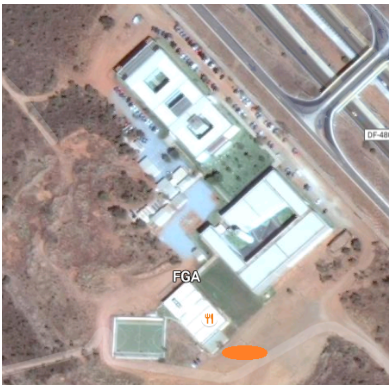
\includegraphics[width=0.75\paperwidth]{figuras/PosicaoBiodigestor.png}
\caption{Foto aérea do campus FGA. Marcação laranja indica o posicionamento do biodigestor}
%\label{Rotulo}
\end{figure}
